\chapter{M. Noirtier de Villefort}

We will now relate what was passing in the house of the king’s attorney
after the departure of Madame Danglars and her daughter, and during the
time of the conversation between Maximilian and Valentine, which we
have just detailed.

M. de Villefort entered his father’s room, followed by Madame de
Villefort. Both of the visitors, after saluting the old man and
speaking to Barrois, a faithful servant, who had been twenty-five years
in his service, took their places on either side of the paralytic.

M. Noirtier was sitting in an armchair, which moved upon casters, in
which he was wheeled into the room in the morning, and in the same way
drawn out again at night. He was placed before a large glass, which
reflected the whole apartment, and so, without any attempt to move,
which would have been impossible, he could see all who entered the room
and everything which was going on around him. M. Noirtier, although
almost as immovable as a corpse, looked at the new-comers with a quick
and intelligent expression, perceiving at once, by their ceremonious
courtesy, that they were come on business of an unexpected and official
character.

Sight and hearing were the only senses remaining, and they, like two
solitary sparks, remained to animate the miserable body which seemed
fit for nothing but the grave; it was only, however, by means of one of
these senses that he could reveal the thoughts and feelings that still
occupied his mind, and the look by which he gave expression to his
inner life was like the distant gleam of a candle which a traveller
sees by night across some desert place, and knows that a living being
dwells beyond the silence and obscurity.

Noirtier’s hair was long and white, and flowed over his shoulders;
while in his eyes, shaded by thick black lashes, was concentrated, as
it often happens with an organ which is used to the exclusion of the
others, all the activity, address, force, and intelligence which were
formerly diffused over his whole body; and so although the movement of
the arm, the sound of the voice, and the agility of the body, were
wanting, the speaking eye sufficed for all. He commanded with it; it
was the medium through which his thanks were conveyed. In short, his
whole appearance produced on the mind the impression of a corpse with
living eyes, and nothing could be more startling than to observe the
expression of anger or joy suddenly lighting up these organs, while the
rest of the rigid and marble-like features were utterly deprived of the
power of participation. Three persons only could understand this
language of the poor paralytic; these were Villefort, Valentine, and
the old servant of whom we have already spoken. But as Villefort saw
his father but seldom, and then only when absolutely obliged, and as he
never took any pains to please or gratify him when he was there, all
the old man’s happiness was centred in his granddaughter. Valentine, by
means of her love, her patience, and her devotion, had learned to read
in Noirtier’s look all the varied feelings which were passing in his
mind. To this dumb language, which was so unintelligible to others, she
answered by throwing her whole soul into the expression of her
countenance, and in this manner were the conversations sustained
between the blooming girl and the helpless invalid, whose body could
scarcely be called a living one, but who, nevertheless, possessed a
fund of knowledge and penetration, united with a will as powerful as
ever although clogged by a body rendered utterly incapable of obeying
its impulses.

Valentine had solved the problem, and was able easily to understand his
thoughts, and to convey her own in return, and, through her untiring
and devoted assiduity, it was seldom that, in the ordinary transactions
of every-day life, she failed to anticipate the wishes of the living,
thinking mind, or the wants of the almost inanimate body.

As to the servant, he had, as we have said, been with his master for
five-and-twenty years, therefore he knew all his habits, and it was
seldom that Noirtier found it necessary to ask for anything, so prompt
was he in administering to all the necessities of the invalid.

Villefort did not need the help of either Valentine or the domestic in
order to carry on with his father the strange conversation which he was
about to begin. As we have said, he perfectly understood the old man’s
vocabulary, and if he did not use it more often, it was only
indifference and \textit{ennui} which prevented him from so doing. He
therefore allowed Valentine to go into the garden, sent away Barrois,
and after having seated himself at his father’s right hand, while
Madame de Villefort placed herself on the left, he addressed him thus:

“I trust you will not be displeased, sir, that Valentine has not come
with us, or that I dismissed Barrois, for our conference will be one
which could not with propriety be carried on in the presence of either.
Madame de Villefort and I have a communication to make to you.”

Noirtier’s face remained perfectly passive during this long preamble,
while, on the contrary, Villefort’s eye was endeavoring to penetrate
into the inmost recesses of the old man’s heart.

“This communication,” continued the procureur, in that cold and
decisive tone which seemed at once to preclude all discussion, “will,
we are sure, meet with your approbation.”

The eye of the invalid still retained that vacancy of expression which
prevented his son from obtaining any knowledge of the feelings which
were passing in his mind; he listened, nothing more.

“Sir,” resumed Villefort, “we are thinking of marrying Valentine.” Had
the old man’s face been moulded in wax it could not have shown less
emotion at this news than was now to be traced there. “The marriage
will take place in less than three months,” said Villefort.

Noirtier’s eye still retained its inanimate expression.

Madame de Villefort now took her part in the conversation and added:

“We thought this news would possess an interest for you, sir, who have
always entertained a great affection for Valentine; it therefore only
now remains for us to tell you the name of the young man for whom she
is destined. It is one of the most desirable connections which could
possibly be formed; he possesses fortune, a high rank in society, and
every personal qualification likely to render Valentine supremely
happy,—his name, moreover, cannot be wholly unknown to you. It is M.
Franz de Quesnel, Baron d’Épinay.”

While his wife was speaking, Villefort had narrowly watched the old
man’s countenance. When Madame de Villefort pronounced the name of
Franz, the pupil of M. Noirtier’s eye began to dilate, and his eyelids
trembled with the same movement that may be perceived on the lips of an
individual about to speak, and he darted a lightning glance at Madame
de Villefort and his son. The procureur, who knew the political hatred
which had formerly existed between M. Noirtier and the elder d’Épinay,
well understood the agitation and anger which the announcement had
produced; but, feigning not to perceive either, he immediately resumed
the narrative begun by his wife.

“Sir,” said he, “you are aware that Valentine is about to enter her
nineteenth year, which renders it important that she should lose no
time in forming a suitable alliance. Nevertheless, you have not been
forgotten in our plans, and we have fully ascertained beforehand that
Valentine’s future husband will consent, not to live in this house, for
that might not be pleasant for the young people, but that you should
live with them; so that you and Valentine, who are so attached to each
other, would not be separated, and you would be able to pursue exactly
the same course of life which you have hitherto done, and thus, instead
of losing, you will be a gainer by the change, as it will secure to you
two children instead of one, to watch over and comfort you.”

\begin{figure}[ht]
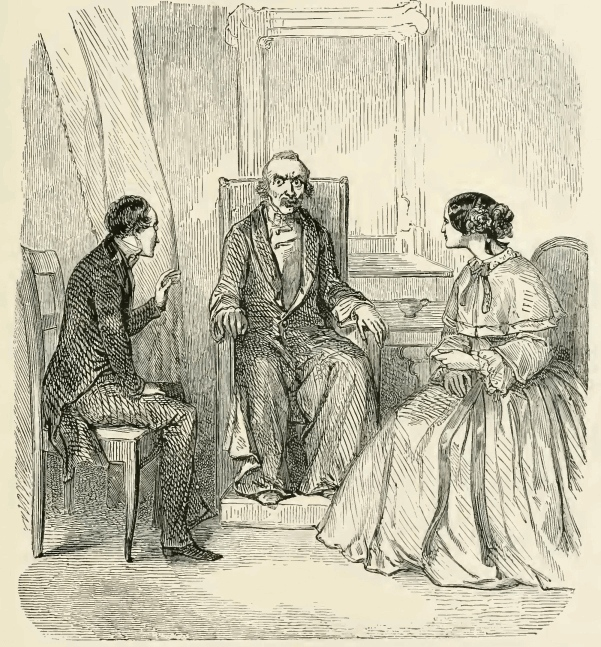
\includegraphics[width=\textwidth]{30165m.jpg}
\end{figure}

Noirtier’s look was furious; it was very evident that something
desperate was passing in the old man’s mind, for a cry of anger and
grief rose in his throat, and not being able to find vent in utterance,
appeared almost to choke him, for his face and lips turned quite purple
with the struggle. Villefort quietly opened a window, saying, “It is
very warm, and the heat affects M. Noirtier.” He then returned to his
place, but did not sit down.

“This marriage,” added Madame de Villefort, “is quite agreeable to the
wishes of M. d’Épinay and his family; besides, he had no relations
nearer than an uncle and aunt, his mother having died at his birth, and
his father having been assassinated in 1815, that is to say, when he
was but two years old; it naturally followed that the child was
permitted to choose his own pursuits, and he has, therefore, seldom
acknowledged any other authority but that of his own will.”

“That assassination was a mysterious affair,” said Villefort, “and the
perpetrators have hitherto escaped detection, although suspicion has
fallen on the head of more than one person.”

Noirtier made such an effort that his lips expanded into a smile.

“Now,” continued Villefort, “those to whom the guilt really belongs, by
whom the crime was committed, on whose heads the justice of man may
probably descend here, and the certain judgment of God hereafter, would
rejoice in the opportunity thus afforded of bestowing such a
peace-offering as Valentine on the son of him whose life they so
ruthlessly destroyed.” Noirtier had succeeded in mastering his emotion
more than could have been deemed possible with such an enfeebled and
shattered frame.

“Yes, I understand,” was the reply contained in his look; and this look
expressed a feeling of strong indignation, mixed with profound
contempt. Villefort fully understood his father’s meaning, and answered
by a slight shrug of his shoulders. He then motioned to his wife to
take leave.

“Now sir,” said Madame de Villefort, “I must bid you farewell. Would
you like me to send Edward to you for a short time?”

It had been agreed that the old man should express his approbation by
closing his eyes, his refusal by winking them several times, and if he
had some desire or feeling to express, he raised them to heaven. If he
wanted Valentine, he closed his right eye only, and if Barrois, the
left. At Madame de Villefort’s proposition he instantly winked his
eyes.

Provoked by a complete refusal, she bit her lip and said, “Then shall I
send Valentine to you?” The old man closed his eyes eagerly, thereby
intimating that such was his wish.

M. and Madame de Villefort bowed and left the room, giving orders that
Valentine should be summoned to her grandfather’s presence, and feeling
sure that she would have much to do to restore calmness to the
perturbed spirit of the invalid. Valentine, with a color still
heightened by emotion, entered the room just after her parents had
quitted it. One look was sufficient to tell her that her grandfather
was suffering, and that there was much on his mind which he was wishing
to communicate to her.

“Dear grandpapa,” cried she, “what has happened? They have vexed you,
and you are angry?”

The paralytic closed his eyes in token of assent.

“Who has displeased you? Is it my father?”

“No.”

“Madame de Villefort?”

“No.”

“Me?” The former sign was repeated.

“Are you displeased with me?” cried Valentine in astonishment. M.
Noirtier again closed his eyes.

“And what have I done, dear grandpapa, that you should be angry with
me?” cried Valentine.

There was no answer, and she continued:

“I have not seen you all day. Has anyone been speaking to you against
me?”

“Yes,” said the old man’s look, with eagerness.

“Let me think a moment. I do assure you, grandpapa—Ah—M. and Madame de
Villefort have just left this room, have they not?”

“Yes.”

“And it was they who told you something which made you angry? What was
it then? May I go and ask them, that I may have the opportunity of
making my peace with you?”

“No, no,” said Noirtier’s look.

“Ah, you frighten me. What can they have said?” and she again tried to
think what it could be.

“Ah, I know,” said she, lowering her voice and going close to the old
man. “They have been speaking of my marriage,—have they not?”

“Yes,” replied the angry look.

“I understand; you are displeased at the silence I have preserved on
the subject. The reason of it was, that they had insisted on my keeping
the matter a secret, and begged me not to tell you anything of it. They
did not even acquaint me with their intentions, and I only discovered
them by chance, that is why I have been so reserved with you, dear
grandpapa. Pray forgive me.”

But there was no look calculated to reassure her; all it seemed to say
was, “It is not only your reserve which afflicts me.”

“What is it, then?” asked the young girl. “Perhaps you think I shall
abandon you, dear grandpapa, and that I shall forget you when I am
married?”

“No.”

“They told you, then, that M. d’Épinay consented to our all living
together?”

“Yes.”

“Then why are you still vexed and grieved?” The old man’s eyes beamed
with an expression of gentle affection.

“Yes, I understand,” said Valentine; “it is because you love me.” The
old man assented.

“And you are afraid I shall be unhappy?”

“Yes.”

“You do not like M. Franz?” The eyes repeated several times, “No, no,
no.”

“Then you are vexed with the engagement?”

“Yes.”

“Well, listen,” said Valentine, throwing herself on her knees, and
putting her arm round her grandfather’s neck, “I am vexed, too, for I
do not love M. Franz d’Épinay.”

An expression of intense joy illumined the old man’s eyes.

“When I wished to retire into a convent, you remember how angry you
were with me?” A tear trembled in the eye of the invalid. “Well,”
continued Valentine, “the reason of my proposing it was that I might
escape this hateful marriage, which drives me to despair.” Noirtier’s
breathing came thick and short.

“Then the idea of this marriage really grieves you too? Ah, if you
could but help me—if we could both together defeat their plan! But you
are unable to oppose them,—you, whose mind is so quick, and whose will
is so firm are nevertheless, as weak and unequal to the contest as I am
myself. Alas, you, who would have been such a powerful protector to me
in the days of your health and strength, can now only sympathize in my
joys and sorrows, without being able to take any active part in them.
However, this is much, and calls for gratitude and Heaven has not taken
away all my blessings when it leaves me your sympathy and kindness.”

At these words there appeared in Noirtier’s eye an expression of such
deep meaning that the young girl thought she could read these words
there: “You are mistaken; I can still do much for you.”

“Do you think you can help me, dear grandpapa?” said Valentine.

“Yes.” Noirtier raised his eyes, it was the sign agreed on between him
and Valentine when he wanted anything.

“What is it you want, dear grandpapa?” said Valentine, and she
endeavored to recall to mind all the things which he would be likely to
need; and as the ideas presented themselves to her mind, she repeated
them aloud, then,—finding that all her efforts elicited nothing but a
constant \textit{“No,”}—she said, “Come, since this plan does not answer, I
will have recourse to another.”

She then recited all the letters of the alphabet from A down to N. When
she arrived at that letter the paralytic made her understand that she
had spoken the initial letter of the thing he wanted.

“Ah,” said Valentine, “the thing you desire begins with the letter N;
it is with N that we have to do, then. Well, let me see, what can you
want that begins with N? Na—Ne—Ni—No——”

“Yes, yes, yes,” said the old man’s eye.

“Ah, it is No, then?”

“Yes.”

Valentine fetched a dictionary, which she placed on a desk before
Noirtier; she opened it, and, seeing that the old man’s eye was
thoroughly fixed on its pages, she ran her finger quickly up and down
the columns. During the six years which had passed since Noirtier first
fell into this sad state, Valentine’s powers of invention had been too
often put to the test not to render her expert in devising expedients
for gaining a knowledge of his wishes, and the constant practice had so
perfected her in the art that she guessed the old man’s meaning as
quickly as if he himself had been able to seek for what he wanted. At
the word \textit{Notary}, Noirtier made a sign to her to stop.

\begin{figure}[ht]
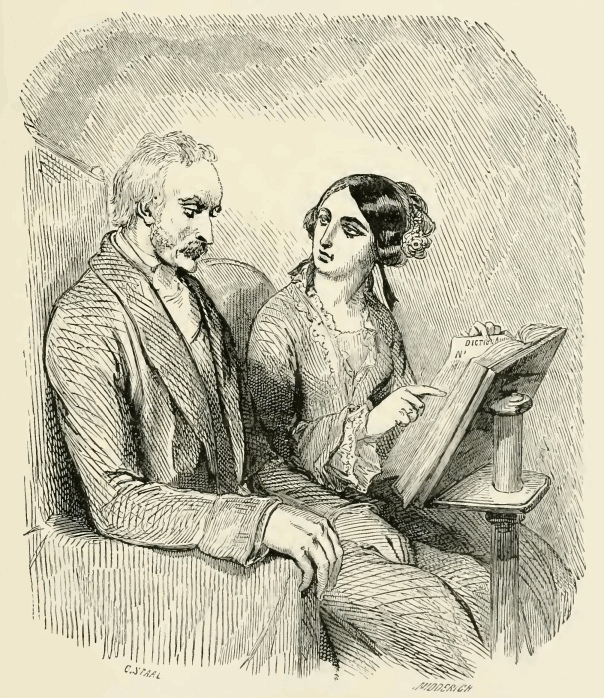
\includegraphics[width=\textwidth]{30169m.jpg}
\end{figure}

“Notary,” said she, “do you want a notary, dear grandpapa?” The old man
again signified that it was a notary he desired.

“You would wish a notary to be sent for then?” said Valentine.

“Yes.”

“Shall my father be informed of your wish?”

“Yes.”

“Do you wish the notary to be sent for immediately?”

“Yes.”

“Then they shall go for him directly, dear grandpapa. Is that all you
want?”

“Yes.” Valentine rang the bell, and ordered the servant to tell
Monsieur or Madame de Villefort that they were requested to come to M.
Noirtier’s room.

“Are you satisfied now?” inquired Valentine.

“Yes.”

“I am sure you are; it is not very difficult to discover that.” And the
young girl smiled on her grandfather, as if he had been a child. M. de
Villefort entered, followed by Barrois.

“What do you want me for, sir?” demanded he of the paralytic.

“Sir,” said Valentine, “my grandfather wishes for a notary.” At this
strange and unexpected demand M. de Villefort and his father exchanged
looks.

“Yes,” motioned the latter, with a firmness which seemed to declare
that with the help of Valentine and his old servant, who both knew what
his wishes were, he was quite prepared to maintain the contest.

“Do you wish for a notary?” asked Villefort.

“Yes.”

“What to do?”

Noirtier made no answer.

“What do you want with a notary?” again repeated Villefort. The
invalid’s eye remained fixed, by which expression he intended to
intimate that his resolution was unalterable.

“Is it to do us some ill turn? Do you think it is worth while?” said
Villefort.

“Still,” said Barrois, with the freedom and fidelity of an old servant,
“if M. Noirtier asks for a notary, I suppose he really wishes for a
notary; therefore I shall go at once and fetch one.” Barrois
acknowledged no master but Noirtier, and never allowed his desires in
any way to be contradicted.

\begin{figure}[ht]
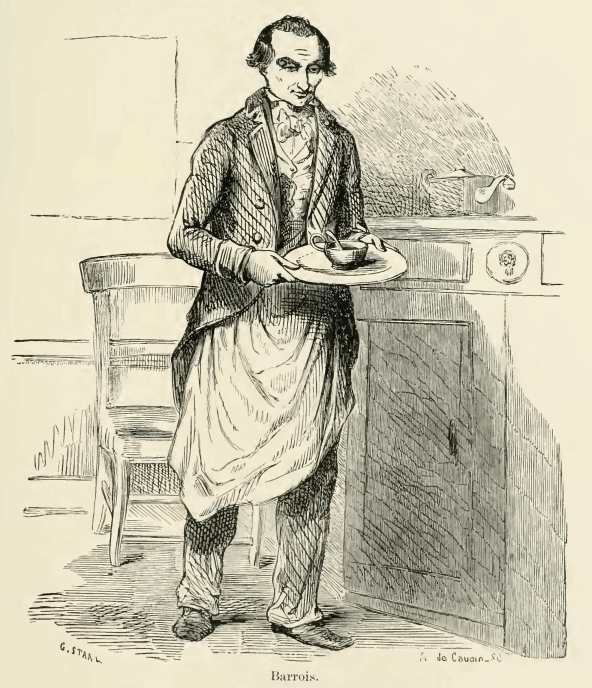
\includegraphics[width=\textwidth]{30171m.jpg}
\end{figure}

“Yes, I do want a notary,” motioned the old man, shutting his eyes with
a look of defiance, which seemed to say, “and I should like to see the
person who dares to refuse my request.”

“You shall have a notary, as you absolutely wish for one, sir,” said
Villefort; “but I shall explain to him your state of health, and make
excuses for you, for the scene cannot fail of being a most ridiculous
one.”

“Never mind that,” said Barrois; “I shall go and fetch a notary,
nevertheless.” And the old servant departed triumphantly on his
mission.
